\rightline{{\rm \textit{Ch-ch-ch-ch-changes}}}
\rightline{{\rm \textit{Turn and face the strange}}}
\rightline{{\rm \textit{Ch-ch-changes}}}
\rightline{{\rm \textit{There's gonna have to be a different man}}}

\rightline{{\rm --- David Bowie}}

In studying fluid motion, we are inherently interested in \textbf{change} in various quantities associated with the fluid. For example, simply because of fluid moving around, its local density or its local temperature might change. With that perspective, the main goal of the science of fluid dynamics is to describe and then calculate that change. Much of the time, we would like to know how flow affects various fluid properties such as its density, pressure, temperature, or even things like mixture composition in multicomponent fluids.
In this Chapter, I discuss the most fundamental building block for talking about change -- \textbf{a derivative}. I hope to show you just how expressive derivatives are in terms of the various types of processes that they can describe!

\section{Derivatives model change}

\textbf{Change} is mathematically modeled by \textbf{derivatives}. A derivative explains how much one variable, say $\varphi$, changes when we change some other variable, say $\psi$, and we express this in mathematical terms as
\begin{equation*}\label{eq:change-d}
\frac{d \varphi}{d \psi} \, ,
\end{equation*}
where the letter $d$ stands for \textit{the change of...} and is later followed by the variable that we are speaking of. So really the above ratio means that there is \textit{this much} change in variable $\varphi$ per \textit{this much} change in variable $\psi$. You can also think of this ratio as \textit{this much} change in variable $\varphi$ per \textit{unit} change in variable $\psi$.

In fluid dynamics, you will find that we are most interested in two types of change: \textit{change in time} and \textit{change in space}. Since we live in a 3D space, with Cartesian coordinates $x$, $y$, and $z$, with a time arrow ($t$), it is justifiable why these two have the biggest popularity, right? Therefore, you will most often encounter $dt$, or $dx$, $dy$, and $dz$, in the denominator of various forms of derivatives.

Let's take pressure, $p$, as an example. When we write
\begin{equation*}\label{eq:change-p}
\frac{d p}{d t} \, ,
\end{equation*}
you can read this as: there is this much change in $p$ per this much change in $t$. Here, we have implicitly assumed that $p = p(t)$, that is, that pressure is only a function of time (and not space).
Similarly, you may encounter expressions like
\begin{equation*}\label{eq:change-p}
\frac{d p}{d x} \,  , \,\, \frac{d p}{d y} \, , \,\, \text{and} \,\, \frac{d p}{d z} \, ,
\end{equation*}
which you can read as: change in $p$ per change in $x$, or $y$, or $z$. 
Here, the assumption was that $p = p(x)$, or $p = p(y)$, or $p = p(z)$, respectively.

The above are what we call \textit{ordinary derivatives}. They assume that the variable can change with respect to only one independent variable. But this does not always need to be the case. 

There is also another mathematical expression for a derivative and it is
\begin{equation*}\label{eq:change-partial}
\frac{\partial \varphi}{\partial \psi} \, .
\end{equation*}
The operator $\partial$ (called ''partial`` or ''del``) also stands for \textit{the change of...} but it also gives you a hint that the variable $\varphi$ can change with the change of variables other than $\psi$. Perhaps it can also change with some $\zeta$ and $\chi$, even though in this particular ratio from above we are only interested in the change with respect to $\psi$.

These are called \textit{partial derivatives}. If a variable is a function of more than one independent variable, say $p = p(x,t)$, we are no longer allowed to use ordinary derivatives to be mathematically precise\footnote{Although we all allow ourselves to be mathematically sloppy sometimes! And that's alright, as long as we remember how to be precise if needed.}. Therefore, if $p = p(x,t)$, and we want to express the change of $p$ with respect to time, we have to write
\begin{equation*}\label{eq:change-partial}
\frac{\partial p}{\partial t}
\end{equation*}
and we can no longer write
\begin{equation*}\label{eq:change-partial}
\frac{d p}{d t} \, .
\end{equation*}


There are what we call \textit{higher-order derivatives}, which can look like this:
\begin{equation*}\label{eq:change-partial-2nd}
\frac{\partial^2 \varphi}{\partial \psi^2} \, .
\end{equation*}
What is their meaning? Well, we can also re-write the above as
\begin{equation*}\label{eq:change-partial}
\frac{\partial}{\partial \psi} \frac{\partial \varphi}{\partial \psi} \, ,
\end{equation*}
and this way it's easier to see that this must have the interpretation of measuring how much the very change in $\varphi$ is changing! In other words, we are describing how the quantity 
\begin{equation*}\label{eq:second-derivative}
\frac{\partial \varphi}{\partial \psi}
\end{equation*}
changes with the change to $\psi$. 

\section{Mixing derivatives signals various transport processes} \label{sec:changes:mixing-derivatives}

The really exciting part begins when we equate derivatives with respect to one quantity to derivatives with respect to other quantity. For instance, we can write that
\begin{equation}\label{eq:dt-propto-dx}
\frac{\partial p}{\partial t} \propto \frac{\partial p}{\partial x}
\end{equation}
for a particular point in space and time, and where the pressure, $p = p(x, t)$.

At first glance, it seems rather bizarre to say that a variable's change in time is proportional to its change in space. In the end, I can imagine a function that varies in space and varies in time, but those variations are completely independent of each other. So what does creating a link between space and time mean...? Let's think about this a little more!

First, we have to come to an agreement where exactly are we measuring $\partial p / \partial t$. With the continuum assumption of fluid dynamics, this is always some point in space, say $Q$. Now that we have selected $Q$, let's look at its local neighborhood to determine how does $p$ vary spatially there. This is what the term $\partial p / \partial x$ describes: How much change in $p$ is there along the spatial $x$-direction? But just the sheer existence of that change does not yet mean that our point $Q$ is going to experience any of it as time goes by! That change simply \textit{is}. If we now wanted it to affect our point $Q$, we need to somehow transport that change over to the location $Q$. And fluid's velocity is a great conveyor of that change! In this case, we have just one spatial dimension, therefore the fluid velocity vector $\vec{\bm{V}} = \langle u \rangle$. If we assume that the velocity component in the $x$-direction, $u$, is the constant of proportionality in Eq.~(\ref{eq:dt-propto-dx}), then we have just described an advection of $p$, which in its full form reads
\begin{equation}\label{eq:advection-of-p}
\frac{\partial p}{\partial t} = - u \frac{\partial p}{\partial x} \, .
\end{equation}
Equating the term $- u \partial p / \partial x$ to the temporal derivative, $\partial p / \partial t$, tells us how much of the spatial change in $p$ is being ``slided over'' to the fixed point in space, $Q$. And the strength of that ``sliding over'' is measured by the velocity component, $u$.

Turns out, the link between time and space, embedded in Eq.~(\ref{eq:advection-of-p}), is necessary when we assume fluid's \textit{movement}. 
As we have seen, a moving fluid can alter a point in time by bringing some spatial change over to that point. Only in the absence of movement can time and space be decoupled and completely independent of one another. It is appreciable that with a relatively simple mathematical description in Eq.~(\ref{eq:advection-of-p}), we have been able to describe this very useful transport phenomena!

A second-order derivative,
\begin{equation*}\label{eq:change-partial-2nd}
\frac{\partial p}{\partial t} = \frac{\partial^2 p}{\partial x^2} \, ,
\end{equation*}
is a model for the \textit{diffusion} of $p$. It describes how much change in $\frac{\partial p}{\partial x}$ are we going to experience along the $x$-direction. While the first-order derivative had the interpretation of how much $p$ is being pushed to the adjacent locations on the $x$-axis, with the second-order derivative we describe what is the strength of that ``pushing'' process.



%\section{What does it mean for a quantity to change in time and in space?}


%\subsection{Steady-state case and a time derivative}

\section{Convention for the sign of a derivative}

For the purpose of this demonstration we will look at the derivative $\frac{dp}{dx}$ -- change in pressure per change in the $x$-axis position -- which is often encountered in fluid dynamics. We will lay the ground for what does it mean for this derivative to be positive, negative or zero, and why the reasoning makes sense.

Suppose that the initial point is marked with \textcolor{myblue}{$(i)$} and it is always a point at coordinate $x$. The point to which we move after one space-step, the final point, is marked with \textcolor{myblue}{$(f)$} and is either at $x+dx$ or $x - dx$ coordinate, depending on the positive or negative change that we decide to make. The direction of the change on the $x$-axis is marked with a blue arrow.

\begin{figure}[H]
\begin{subfigure}[t]{.46\textwidth}
\centering
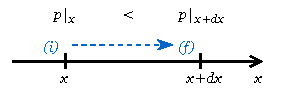
\includegraphics[scale=1]{dp-dx-pos-neg.pdf}
\caption{$\frac{dp}{dx} > 0$ with positive change in $x$.}
\end{subfigure}
\begin{minipage}[t]{.07\textwidth}
$ $
\vspace*{1.5cm}
\end{minipage}
\begin{subfigure}[t]{.46\textwidth}
\centering
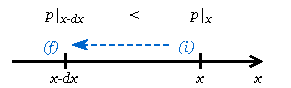
\includegraphics[scale=1]{dp-dx-neg-neg.pdf}
\caption{$\frac{dp}{dx} > 0$ with negative change in $x$.}
\end{subfigure}
\begin{subfigure}[t]{.46\textwidth}
\centering
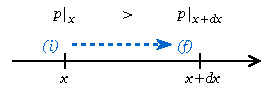
\includegraphics[scale=1]{dp-dx-pos-pos.pdf}
\caption{$\frac{dp}{dx} < 0$ with positive change in $x$.}
\end{subfigure}
\begin{minipage}[t]{.08\textwidth}
$ $
\end{minipage}
\begin{subfigure}[t]{.46\textwidth}
\centering
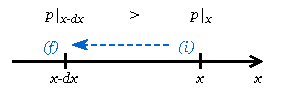
\includegraphics[scale=1]{dp-dx-neg-pos.pdf}
\caption{$\frac{dp}{dx} < 0$ with negative change in $x$.}
\end{subfigure}
\caption{Sign of the $\frac{dp}{dx}$ derivative versus directions of change along the $x$-axis.}
\label{fig:dp-dx-signs}
\end{figure}

We will now find out for all cases which pressure, at \textcolor{myblue}{$(i)$} or at \textcolor{myblue}{$(f)$} must be larger. Our aim is to show that situations (a) and (b) in Figure \ref{fig:dp-dx-signs} must be equivalent -- they explain the same physical phenomena. In both of these cases we will show that the pressure is increasing with the increasing $x$-coordinate, independent of whether we decide to take a step to the right or to the left of our initial point \textcolor{myblue}{$(i)$}. 

We will show the analogical result can be said about situations (c) and (d) but in this case the pressure is decreasing with the increasing $x$-coordinate.

The analysis done in this section is often necessary in order to find out whether or not to ''put a minus sign`` in front of expressions. For instance, as we will show later in the text, such reasoning can help us understand why there is a minus sign in the Euler equation for a fluid element experiencing pressure force: $dp = - \rho \upsilon d \upsilon$. Oftentimes, the sign of a derivative tells an important information about the nature of the physical phenomena.

